\chapter{Introducción}\label{capIntroduccion}

\section{Introducción y motivación}\label{sec:intro}


La principal motivación para la realización de esta memoria es la de cumplir con los requisitos necesarios para presentar el trabajo de fin de grado del grado en Ingeniería Informática - Tecnologías Informáticas aunque obviamente también existe la motivación personal del autor de documentar extensivamente el trabajo realizado así como la de profundizar en el área de los sistemas de ayuda a la conducción y, en general en la tecnología a bordo de los vehículos de hoy dia.


\section{Estructura de esta memoria} \label{sec:estructuramemoria}
Esta memoria se encuentra estructurada en varios bloques:

\begin{itemize}
    \item \textbf{Bloque 1:} Introducción\\
        En este primer bloque se introduce el proyecto así como la temática general en la que se va a centrar. Además también se indicarán los objetivos, tanto técnicos como académicos que se esperan cumplir.

    \item \textbf{Bloque 2:} Ejecución del proyecto\\
        A continuación nos encontraremos con el bloque dedicado a la explicación exhaustiva del diseño e implementación del sistema así como de las pruebas realizadas.

    \item \textbf{Bloque 3:} Planificación del proyecto\\
        En este bloque se tratará la planificación temporal y financiera de este proyecto tanto la planeada inicialmente como los resultados finales tras la elaboración completa del trabajo. 

    \item \textbf{Bloque 4:} Conclusiones\\
        Tras las explicaciones anteriores, en esta sección se remarcarán los objetivos cumplidos así como una pequeña conclusión personal.

    \item \textbf{Bloque 5:} Trabajo futuro\\
        En este bloque se tratarán algunos aspectos cuya ampliación en el futuro creemos que es un aspecto interesante.

    \item \textbf{Referencias bibliográficas y apéndices}\\
        Finalmente nos encontraremos con las referencias bibliográficas y los distintos apéndices de este proyecto.
\end{itemize}


\section{Objetivos del proyecto}\label{sec:Objetivos}

Como para cualquier proyecto será necesario proponer unos objetivos que nos permitan llevar una evaluación del progreso.

\subsection{Objetivos técnicos}
Respecto a objetivos técnicos creemos conveniente que se cumplan los siguientes para dar por finalizado este trabajo.

\begin{itemize}
    \item \textbf{Objetivo 1:} Detección y seguimiento del límite de velocidad
    \item \textbf{Objetivo 2:} Detección y aviso cambio de semáforo
    \item \textbf{Objetivo 3:} Detección y aviso de salida de carril
    \item \textbf{Objetivo 4:} Detección y aviso de vehículos en angulo muerto
    \item \textbf{Objetivo 5:} Detección y aviso de peatones en la trayectoria del vehículo
    \item \textbf{Objetivo 6:} Satisfactoria implementación del sistema en un sistema empotrado
\end{itemize}

A modo de resumen, como objetivo general que englobe a todos los demás se puede considerar el diseño e implementación de un sistema integral de ayuda a la conducción basado en sistemas empotrados de bajo coste que sea capaz de detectar situaciones y estados anómalos y notifique al conductor de forma visual y auditiva.

\subsection{Objetivos académicos}
Además de los objetivos técnicos enunciados en la sección anterior también se podrán considerar una serie de requisitos distintos relacionados con el carácter educativo y académico de este proyecto.

La elaboración de este trabajo no es más que el culmen final del trabajo realizado durante todos los años de estudios por lo que es natural que nos planteemos los siguientes objetivos que nos permitan demostrar y ampliar nuestro conocimiento en esta materia.

\begin{itemize}
    \item \textbf{Objetivo 1:} Creación de una aplicación robusta y funcional que cumpla los objetivos técnicos especificados con anterioridad
    \item \textbf{Objetivo 2:} Ampliar conocimiento y profundizar en el estudio de distintas técnicas de \textit{Machine Learning}
    \item \textbf{Objetivo 3:} Ampliar conocimiento sobre la elaboración de aplicaciones con interfaz de usuario gráfica
\end{itemize}



\section{Estado del arte}\label{sec:stateoftheart}

El sistema que proponemos no es algo novel ya que actualmente existen tanto soluciones similares como soluciones mucho más complejas y completas en el mercado.

En los últimos años se ha producido una gran explosión en la investigación y comercialización de estos sistemas debido a las peticiones de los clientes que desean más seguridad para sus familias y que tienen la mirada puesta en la eventual conversión a la conducción autónoma total.

Los sistemas de ayuda a la conducción han sido unos de los primeros pasos que se han dado en la búsqueda de la conducción autónoma por parte de las empresas automovilísticas. Así pues nos podemos encontrar con sistemas como Mobileye\cite{yoffie2014mobileye}, que forman la base de sistemas de ayuda a la conducción como Nissan ProPilot y las primeras versiones del sistema Autopilot de Tesla.

Empresas como Waymo y Uber también han creado sistemas de conducción autónoma con sensores LIDAR que obtienen una nube de puntos de alta resolución de los alrededores del vehículo.
Además, existen otros sistemas basados en visión por computador creados por las propias empresas automovilísticas como SuperCruise de Caddillac, que consigue navegar en autopistas sin problema alguno gracias a la ayuda de \textit{HD maps} generados previamente\cite{CaddillacSupercruise}, o las últimas versiones del sistema Autopilot de Tesla \cite{teslaAutopilot}, que alcanza un nivel de autonomía 2 en cualquier tipo de calzada con marcas claramente visibles.

SuperCruise es uno de los ejemplos más interesantes en cuanto al control del conductor ya que gracias a una serie de sensores situados en el volante son capaces de vigilar la atención del conductor. El uso de estos sensores es mucho mas avanzado que el simple sensor de fuerza de torsión que usa Tesla para la misma función, aunque cabe destacar que los últimos modelos de la marca (Model 3 y Model Y) incorporan una cámara que tiene visión del interior del vehículo \cite{manualModel3} así que es muy posible que en el futuro cercano se comience a utilizar para vigilar al conductor mediante el uso de visión por computador.

El ejemplo que más se parece a nuestro proyecto sería OpenPilot, de Comma.ai \cite{openpilot}, un proyecto basado en visión por computador e inteligencia artificial que, junto con los datos del radar de los vehículos compatibles, es capaz de analizar el entorno y controlar el vehículo hasta un nivel 2 de autonomía.

Por supuesto, a pesar de ser el sistema más parecido al propuesto, nuestro sistema quedará lejos de este otro pues la capacidad tecnológica del autor no podrá ser comparada con la del grupo de personas que desarrollan OpenPilot.


\subsection{Tesla Autopilot}

El sistema Tesla Autopilot es el sistema de conducción autónoma de nivel 2 disponible para la mayoría de vehículos creados por la empresa estadounidense y que ofrece la capacidad de controlar el vehículo en diversos entornos.
La recolección de datos se centra principalmente en las imágenes obtenidas por las cámaras del vehículo aunque también se trata la información generada por el radar central y los sensores de ultrasonidos.

En diversas conferencias Andrej Karpathy ha compartido detalles sobre el funcionamiento interno de este sistema y como este ha ido evolucionando para, con el tiempo, ir convirtiéndose en un sistema mucho más centrado en los sistemas de inteligencia artificial.

El sistema autopilot está compuesto por más de 48 redes neuronales que realizan más de 1000 predicciones por cada fotograma analizado. Uno de los sistemas más interesantes es el sistema de predicción de calzada en vista cenital que se puede observar en la figura \ref{fig:preditorCalzadasTesla}. Este sistema es capaz de generar un mapa bidimensional del entorno alrededor del vehículo con un precisión bastante acertada utilizando únicamente los datos obtenidos por la cámaras del vehículo \cite{teslaAutonomyDay} \cite{karpathyAI} \cite{karpathyPytorch}.

Una parte de nuestro trabajo, tal y como se verá en el siguiente capítulo, esta inspirada en este sistema.

\begin{figure}[h!]
    \begin{subfigure}[c]{.5\textwidth}
      \centering
      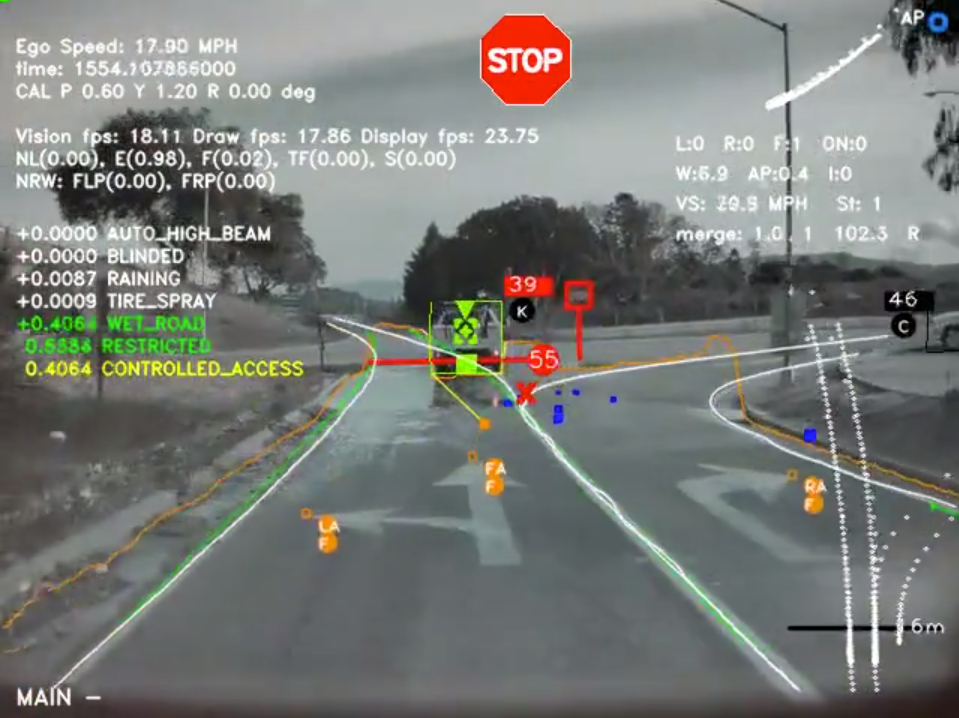
\includegraphics[width=.8\linewidth]{img/teslaautopilotOverlays.png}
      \caption{Fotograma de un video que muestra el comportamiento interno del sistema \textit{autopilot} de los vehículos Tesla}
      \label{fig:teslaautopilotvideorecruit}
    \end{subfigure}%
    \begin{subfigure}[c]{.5\textwidth}
      \centering
      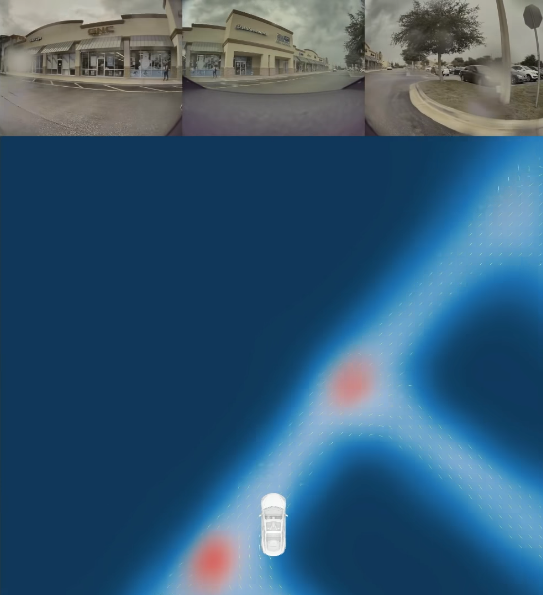
\includegraphics[width=.8\linewidth]{img/teslaTopDown.png}
      \caption{Salida del predictor de calzadas en la vista cenital}
      \label{fig:preditorCalzadasTesla}
    \end{subfigure}
    
    \caption{Ejemplos del funcionamiento interno del sistema Tesla Autopilot}
    \label{fig:ejemploTesla}
\end{figure}

\subsection{Caddillac SuperCruise}

En cuanto al sistema de conducción semiautónoma de Cadillac, SuperCruise, se puede destacar que es un sistema que utiliza mapas de alta resolución generados mediante LIDAR, Radar, GPS y cámaras convencionales para permitir que el vehículo pueda conducir sin la interacción directa del conductor \cite{CaddillacSupercruise}. 

A pesar de que apenas existe información sobre este sistema, ya que tan solo se puede utilizar en varias autopistas de EEUU y Canadá y que la cantidad de personas con acceso a él es mucho menor que a la de los sitemas de sus competidores, en la figura \ref{fig:cadillactobii} se puede observar el dispositivo encargado de controlar la atención del conductor que, ademas de un led indicador, parece tener 6 leds infrarrojos que proyectarán un patrón fácilmente reconocible en la pupila del conductor. Este sistema, parece tener gran similitud con los sistemas de seguimiento ocular para consumidores de la empresa Tobii, uno de los cuales será utilizado en este proyecto.

\begin{figure}[h!]
    \centering
    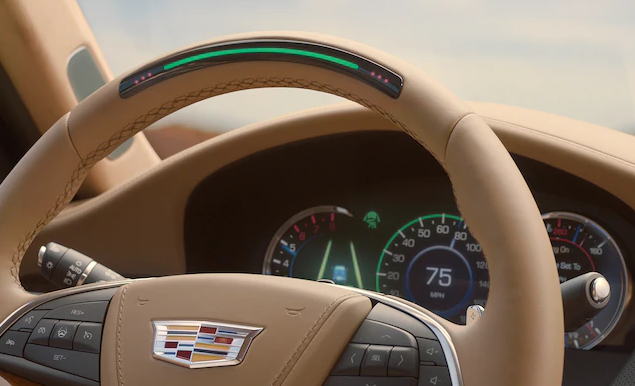
\includegraphics[width=.7\linewidth]{img/cadillacSupercruise.png}
    \caption{Detalle del sistema de control del conductor de Caddillac Supercruise}
    \label{fig:cadillactobii}
\end{figure}

\subsection{OpenPilot}

Openpilot es un sistema de conducción autónoma open-source desarrollado por George Hotz capaz de detectar las líneas de la calzada e interaccionar con el radar de los vehículos compatibles para controlarlo hasta un nivel de autonomía 2. Además también realiza alertas visuales y auditivas ante situaciones anómalas, como por ejemplo la superación del límite de velocidad.
Inicialmente, el sistema se ejecutaba en un teléfono móvil convencional pero posteriormente se ha trasladado a una solución hardware propietaria.

Uno de los puntos interesantes de esta solución es la compatibilidad con más de 85 vehículos de distintas marcas, algo solo posible al tratarse de un proyecto \textit{opensource}.

\begin{figure}[h!]
    \begin{subfigure}[c]{.5\textwidth}
      \centering
      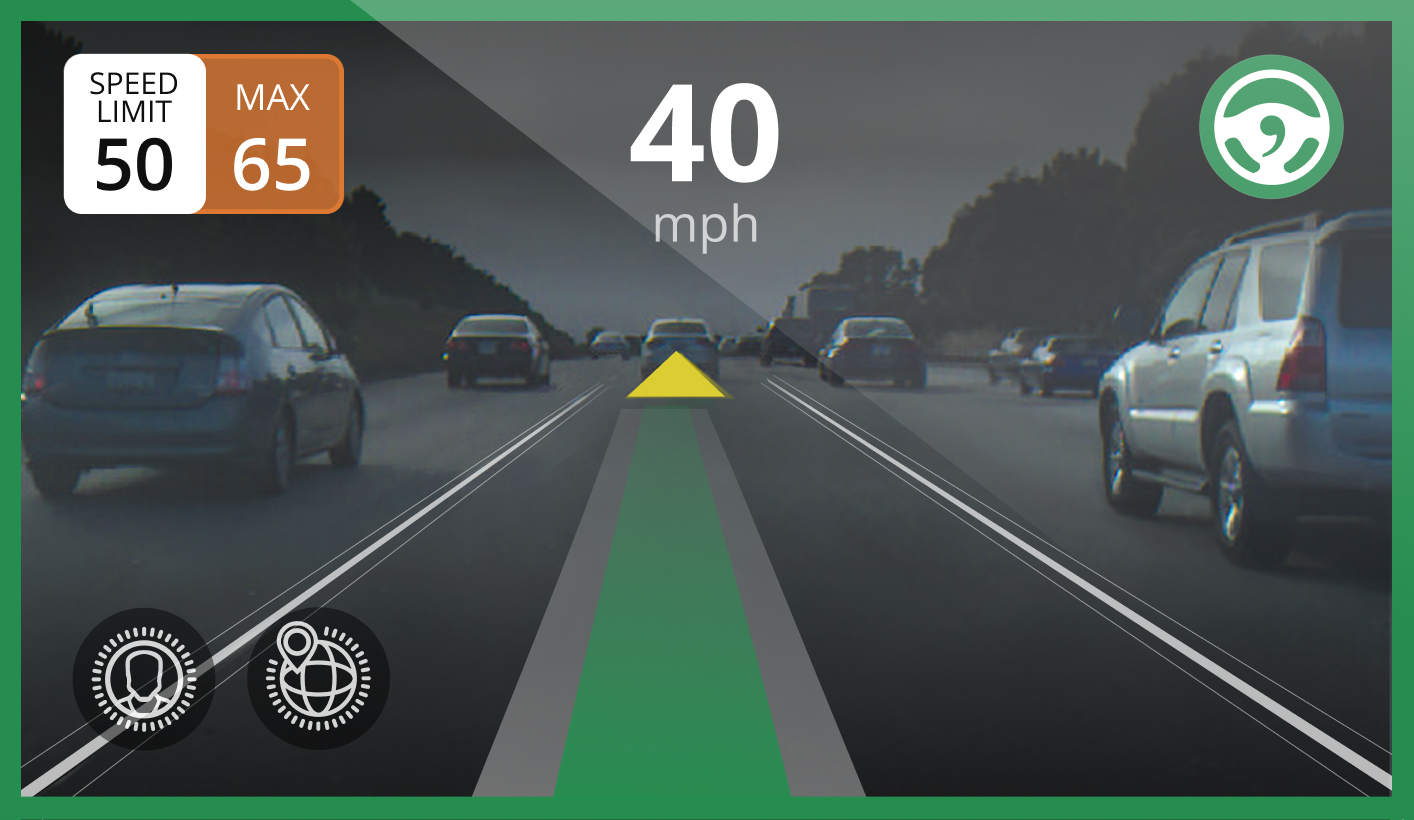
\includegraphics[width=.8\linewidth]{img/Openpilot.jpg}
      \caption{Interfaz gráfica del sistema Openpilot}
      \label{fig:openpilot1}
    \end{subfigure}%
    \begin{subfigure}[c]{.5\textwidth}
      \centering
      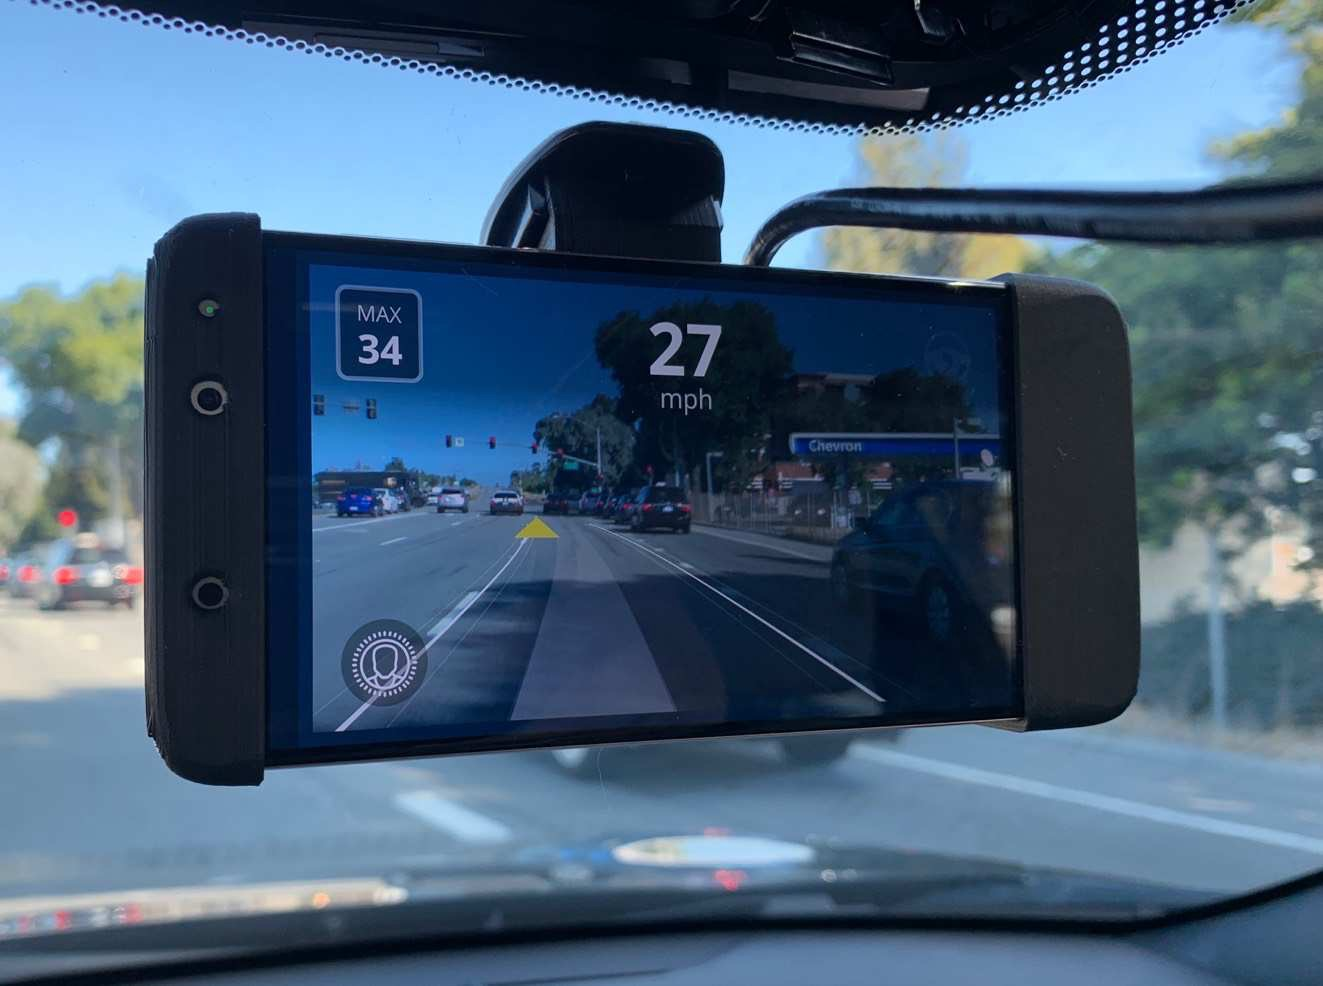
\includegraphics[width=.8\linewidth]{img/openpilot2.jpeg}
      \caption{Ejemplo de uso de Openpilot en un vehículo real}
      \label{fig:openpilot2}
    \end{subfigure}
    
    \caption{Ejemplos del funcionamiento del sistema Openpilot}
    \label{fig:ejemploOpenpilot}
\end{figure}

\section{Elicitación de requisitos}\label{sec:requisitos}

A continuación se indican los requisitos que nuestra aplicación deberá cumplir para considerar una entrega final como satisfactoria.

\begin{itemize}
    \item El sistema deberá recibir la información del vehículo y mostrarla
    \item El sistema deberá ser capaz de reconocer los vehículos a su alrededor
    \item El sistema deberá detectar los cambios de los semáforos
    \item El sistema deberá controlar la atención del conductor
    \item El sistema deberá avisar acústica y visualmente ante situaciones anómalas
\end{itemize}


\section{Análisis de riesgos} \label{sec:analisisriesgos}

Por supuesto, como cualquier otro proyecto es posible que se den algunos problemas. A continuación se describen los posibles riesgos que se pueden dar.

\subsection{Identificación de los posibles riesgos}

\begin{itemize}
    \item Posibles retrasos derivados de las distintas obligaciones del autor\\
        Puesto que la elaboración de este proyecto se realizará en paralelo a la finalización de los estudios del autor y de la entrada al mundo laboral es bastante posible que la priorización de otras tareas no relacionadas con la ejecución del proyecto afecten a los tiempos de desarrollo del mismo.

    \item Pérdida parcial o completa del código fuente\\
        Al trabajar con un proyecto importante siempre es preocupante que debido a problemas de hardware se produzca la pérdida parcial o completa del código fuente.

    \item Imposibilidad del acceso a las herramientas de desarrollo\\
        Otro de los posibles problemas que nos podemos encontrar será la imposibilidad de acceder a las herramientas de desarrollo de nuestro proyecto por causas de fuerza mayor.

    \item Dificultad de implementación\\
        Otro posible riesgo que nos podemos encontrar sería las posibles complicaciones durante la implementación de alguna parte del proyecto. Estas complicaciones podrían aparecer a raíz del desconocimiento de algún tipo de herramienta o librería por parte de los autores.

\end{itemize}

\subsection{Plan de contingencia ante los posibles riesgos}
En el caso de que alguno de los riesgos enunciados anteriormente llegue a materializarse es conveniente conocer las distintas opciones disponibles para minimizar las partes del trabajo que se verían afectadas.

\begin{itemize}
    \item Retrasos en la elaboración del proyecto\\
        La principal solución a los problemas de retrasos consistirá en la reorganización de las tareas y, en el caso de que sea necesario, el retraso de la entrega a las distintas convocatorias disponibles durante el curso escolar.

    \item Pérdida del código fuente\\
        La perdida del código fuente supondría el aplazamiento completo de las tareas y consecuentes retrasos por lo que este es un riesgo que no podemos permitirnos. Afortunadamente, en nuestra industria, la perdida parcial o completa es un riesgo menor gracias a los distintos sistemas que existen para llevar un seguimiento de datos. Para reducir este riesgo y que nunca se llegue a dar, todo el código utilizado en este proyecto se encuentra archivado siguiendo la regla copias de seguridad 321 \cite{backups321}. En concreto, para nuestro proyecto existen al menos 5 copias en 2 medios distintos y con al menos 2 copias \textit{offsite}.

    \item Imposibilidad del acceso a las herramientas de desarrollo\\
        En el caso de que perdamos el acceso a las herramientas de desarrollo de nuestro proyecto o no podamos acceder a ellas por causas de fuerza mayor deberemos modificar la planificación para intentar que el periodo durante el que no tengamos acceso se pueda invertir en otras tareas que no dependan de estas herramientas. Aun así, si este riesgo llegase a materializarse se deberá aceptar el hecho de que los retrasos serán necesarios.
            
    \item Dificultad de implementación\\
        En el caso de que nos encontremos con distintos problemas durante la implementación de alguna parte del proyecto nos veremos obligados a realizar una extensiva investigación para resolver los problemas con los que nos podamos encontrar. Afortunadamente tanto las herramientas como el hardware utilizados parecen estar muy bien documentados y tienen una gran comunidad de personas detrás que nos permitirán, casi con total seguridad, encontrar las respuestas a nuestras preguntas. Si los frutos de la investigación no son suficientes siempre podremos apoyarnos en la ayuda que nuestros tutores nos puedan aportar.

\end{itemize}